\documentclass[12pt,a4paper]{article}
\usepackage[a4paper, margin=2cm]{geometry}
\usepackage{amsmath}
\usepackage{fancyhdr}
\usepackage{graphicx}
\usepackage{pdflscape}
\usepackage{svg}
\usepackage{hyperref}
\usepackage{enumitem}
\usepackage[absolute,overlay]{textpos}
\usepackage{lipsum}
\usepackage{amssymb}

\usepackage[portuguese]{babel}
\usepackage{lmodern}
\renewcommand*{\familydefault}{\sfdefault}
\usepackage{geometry}
\usepackage{setspace}
\usepackage{xcolor}
\usepackage{tikz}
\definecolor{col1}{RGB}{0,160,255}
\definecolor{col2}{RGB}{7,74,163}
\usepackage{setspace}
\usepackage{listings}
\usepackage{titlesec}
\usepackage{color}
\usepackage{textgreek}

\newcommand{\reporttitle}{Projeto Computacional - 2.ª Parte}
\newcommand{\authorgroup}{Grupo 16 - Afonso Ribeiro, Diogo Rodrigues, Pedro Mendes}
\newcommand{\istul}{Instituto Superior Técnico -- Universidade de Lisboa}
\newcommand{\reportcourse}{Matemática Experimental}
\newcommand{\reportyear}{2024/2025}

\newcommand{\m}[1]{\mathbf{#1}}

\hypersetup{
    colorlinks=true,
    linkcolor=blue,
    filecolor=magenta,
    urlcolor=blue,
    citecolor=blue,
    pdftitle={\reporttitle},
    pdfpagemode=FullScreen,
}

\pagestyle{fancy}
\fancyhf{}
\lhead{\reporttitle}
\rhead{\reportcourse}
\lfoot{\authorgroup}
\rfoot{\thepage}


\renewcommand{\footrulewidth}{0.2pt}

\renewcommand\thesection{\arabic{section}.}
\renewcommand\thesubsection{\thesection\arabic{subsection}.}
\renewcommand\thesubsubsection{\thesubsection\arabic{subsubsection}.}

\usepackage{etoolbox} % Necessário para modificar comandos
\makeatletter % Indentar parágrafos dentro de subseções
\preto\subsection{\setlength{\parindent}{2em}} % Ajusta o tamanho do recuo
\makeatother

\begin{document}
    \begin{titlepage}
        \thispagestyle{empty}
        \newgeometry{left=2cm, right=1.5cm, top = 2cm, bottom=2cm}
        \begin{tikzpicture}[overlay, fill opacity=0.7]
        \fill[col1] (12,-27) rectangle (15,4);
        \rotatebox{-45}{\fill[col2] (12, -23) rectangle (21,20);}
        \node[anchor=base, color=white] at (13.50, 0) {\Huge \textbf{M}};
        \node[anchor=base, color=white] at (13.50, -1) {\Huge \textbf{A}};
        \node[anchor=base, color=white] at (13.50, -2) {\Huge \textbf{T}};
        \node[anchor=base, color=white] at (13.50, -3) {\Huge \textbf{E}};
        \node[anchor=base, color=white] at (13.50, -4) {\huge \textbf{M}};
        \node[anchor=base, color=white] at (13.50, -5) {\huge \textbf{Á}};
        \node[anchor=base, color=white] at (13.50, -6) {\Huge \textbf{T}};
        \node[anchor=base, color=white] at (13.50, -7) {\Huge \textbf{I}};
        \node[anchor=base, color=white] at (13.50, -8) {\Huge \textbf{C}};
        \node[anchor=base, color=white] at (13.50, -9) {\Huge \textbf{A}};
        \node[anchor=base] at (13.50, -11.7) {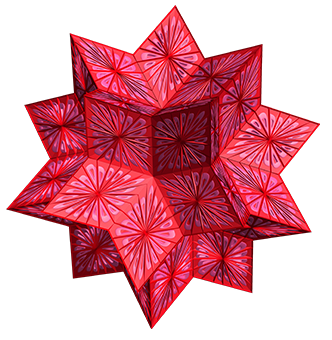
\includegraphics[width=2cm]{Mathematica.png}};
        \node[anchor=base, color=white] at (13.50, -13) {\Huge \textbf{E}};
        \node[anchor=base, color=white] at (13.50, -14) {\Huge \textbf{X}};
        \node[anchor=base, color=white] at (13.50, -15) {\Huge \textbf{P}};
        \node[anchor=base, color=white] at (13.50, -16) {\Huge \textbf{E}};
        \node[anchor=base, color=white] at (13.50, -17) {\Huge \textbf{R}};
        \node[anchor=base, color=white] at (13.50, -18) {\Huge \textbf{I}};
        \node[anchor=base, color=white] at (13.50, -19) {\huge \textbf{M}};
        \node[anchor=base, color=white] at (13.50, -20) {\Huge \textbf{E}};
        \node[anchor=base, color=white] at (13.50, -21) {\Huge \textbf{N}};
        \node[anchor=base, color=white] at (13.50, -22) {\Huge \textbf{T}};
        \node[anchor=base, color=white] at (13.50, -23) {\Huge \textbf{A}};
        \node[anchor=base, color=white] at (13.50, -24) {\Huge \textbf{L}};
        
        \node[anchor=center, color=black, rotate=45] at (5, -10.9) {\Huge \textbf{RELATÓRIO}};
        \end{tikzpicture}
        \begin{spacing}{1.5}
        \begin{flushleft}
        {\Huge \textbf{Projeto Computacional}}\\ [10pt]
        {\huge  \textbf{2.ª Parte}}\\ [48pt]
        {
\includegraphics[scale=0.40]{IST_Logo.png}} \\ [1.5cm]
        \end{flushleft}
        \end{spacing}
        \begin{minipage}{2cm}
        \end{minipage} 
        \vspace{6.4 cm}
        \begin{flushleft}
        
        \Large \textcolor{white}{
            Trabalho realizado por: \\
            Afonso Ribeiro, ist1102763 \\
            Diogo Rodrigues, ist1113787 \\
            Pedro Mendes, ist1109994 \\
            \vspace{0.5cm} \\
            Com o apoio dos professores: \\
            Pedro Lima \\
            André Crispim
        }
        \end{flushleft}
        \vspace{1cm}
     \end{titlepage}

    \setcounter{page}{2}
    \setcounter{secnumdepth}{0} % Disable numbering for sections and below
    \setlength{\parskip}{0em}

    \newlength{\imagewidth} % Declare a new length
    \setlength{\imagewidth}{8cm} % Set its value


    \section{1. Frações contínuas e constante de Khinchin}
    \subsection{a)}
        \begin{itemize}
            \item Esta função aproxima a constante de Khinchin (\(\approx 2.68545\)) através do produto infinito:
            \[
            K_0 \;=\;
            \prod_{k=1}^{\infty}\Bigl(1 + \tfrac{1}{k(k+2)}\Bigr)^{\log_2(k)}.
            \]
            \item O parâmetro \(\texttt{epsilon}\) especifica a tolerância para o erro absoluto.
            \item A cada iteração, calcula-se o próximo fator \(\bigl(1 + 1/[k(k+2)]\bigr)^{\log_2(k)}\), multiplica-se ao produto parcial, e verifica-se se a diferença \(|\texttt{produtoParcial} - K_0|\) é menor que \(\epsilon\).
            \item Quando o \(\texttt{If}\) deteta que o erro ficou abaixo de \(\epsilon\), a função retorna o valor do produto e o número de fatores \(k\) necessários.
        \end{itemize}
    
    \subsection{b)}
        \begin{itemize}
            \item Esta função calcula a constante de Khinchin a partir da fração contínua de um número real.
            \item A ideia baseia-se no limite:
            \[
            K_0 \;=\; \lim_{n \to \infty} \bigl(a_1 a_2 \cdots a_n\bigr)^{1/n},
            \]
            onde \(a_1,a_2,\dots\) são os coeficientes da fração contínua (ignorando o termo inicial \(a_0\)).
            \item A função extrai muitos coeficientes via \texttt{ContinuedFraction[x, ...]} e depois acumula o produto dos \(a_i\), calcula a média geométrica, e compara-a com o valor de referência \(\texttt{Khinchin}\).
            \item Se \(|\texttt{geom} - K_0|<\epsilon\), retorna o valor e o número \(n\) de coeficientes usados. Caso contrário, após esgotar o número máximo de coeficientes, imprime uma mensagem de erro.
        \end{itemize}

    
    \subsection{c)}
        \begin{itemize}
            \item \(\pi\): A chamada à função \texttt{khinchin2[\(\pi, \epsilon\)]}, para os valores de \(\epsilon\) na lista \texttt{\{0.1, 0.01, 0.001, 0.0001\}} devolveu valores sucessivamente mais próximos da constante de Khinchin.
            \item \texttt{e}: A chamada à função \texttt{khinchin2[e, 0.01]} devolveu um valor próximo da constante de Khinchin, mas a chamada \texttt{khinchin2[e, 0.001]} falhou.
            \item \texttt{ln(2)}: A chamada à função \texttt{khinchin2[ln(2), \(\epsilon\)]}, para os valores de \(\epsilon\) na lista \texttt{\{0.1, 0.01, 0.001, 0.0001\}} devolveu valores sucessivamente mais próximos da constante de Khinchin.
            \item \(\frac{1+\sqrt{5}}{2}\): A chamada à função \texttt{khinchin2[\(\frac{1+\sqrt{5}}{2}\), 0.001]} falhou.
            \item \(\frac{\sqrt{3}+1}{2}\): A chamada à função \texttt{khinchin2[\(\frac{\sqrt{3}+1}{2}\), 0.001]} falhou.
            \item \(2^{\frac{1}{3}}\): A chamada à função \texttt{khinchin2[\(2^{\frac{1}{3}}, \epsilon\)]}, para os valores de \(\epsilon\) na lista \texttt{\{0.1, 0.01, 0.001, 0.0001\}} devolveu valores sucessivamente mais próximos da constante de Khinchin.
            \item \(e^\pi\): A chamada à função \texttt{khinchin2[\(e^\pi, \epsilon\)]}, para os valores de \(\epsilon\) na lista \texttt{\{0.1, 0.01, 0.001, 0.0001\}} devolveu valores sucessivamente mais próximos da constante de Khinchin.
            \item \texttt{sin(1)}: A chamada à função \texttt{khinchin2[sin(1), \(\epsilon\)]}, para os valores de \(\epsilon\) na lista \texttt{\{0.1, 0.01, 0.001, 0.0001\}} devolveu valores sucessivamente mais próximos da constante de Khinchin.
            \item \texttt{tan(1/2)}: A chamada à função \texttt{khinchin2[tan(1/2), 0.1]} devolveu um valor próximo da constante de Khinchin, mas a chamada \texttt{khinchin2[tan(1/2), 0.01]} falhou.
        \end{itemize}

        Verifica-se, então, que, para os números \(\pi\), \texttt{ln(2)}, \(2^{\frac{1}{3}}\), \(e^\pi\) e \texttt{sin(1)}, o limite converge para a constante de Khinchin. No entanto, era expectável que, para os valores \texttt{e} e \texttt{tan(1/2)}, o limite convergisse, formulando-se a conjetura de que somente para números racionais e irracionais quadráticos o limite não converge para a constante de Khinchin, e que para todos os demais (transcendentes e algébricos de grau \(\geq\) 3) converge. Estes dois valores de \(x\) obtiveram um resultado próximo da constante pretendida para valores mais altos de \(\epsilon\), falhando depois com valores mais baixos. Esta falha poderá estar relacionada com a necessidade de obter os resultados com um maior número de elementos nas frações contínuas dos números em questão, o que não nos foi possível, pois a computação da função \texttt{khinchin2} não terminava em tempo útil nessas condições.

    \subsection{d)}
        Para cada um dos valores de \(\epsilon\) especificados, os valores de \(k_{max}\) para o comando \texttt{khinchin1} e de \(n_{max}\) para o comando \texttt{khinchin2} com \(x = \pi\) e \(x = \sin(1)\) foram, respetivamente, os seguintes.
        \[\begin{array}{c|ccc}
            \epsilon & k_{\max} & n_{\max} (x=\pi) & n_{\max}(x=\sin(1)) \\
            \hline
            10^{-1} & 246 & 16 & 4 \\
            10^{-2} & 3547 & 17 & 57 \\
            10^{-3} & 45411 & 117 & 327 \\
            10^{-4} & 550885 & 976 & 1627 \\
        \end{array}\]
        Discussão da eficiência dos métodos utilizados:
        \begin{itemize}
        \item \textbf{Método \texttt{khinchin1} (produto infinito)}: 
            É um método universal, isto é, não depende de um número \(x\): uma vez implementado, aproxima a constante de Khinchin sem nenhuma informação adicional. Podemos observar na tabela que, para alcançar precisões como \(10^{-3}\) ou \(10^{-4}\), o número de fatores \(k_{\max}\) se torna muito grande (\(45411\) e \(550885\), respectivamente). Portanto, em termos de iterações, este método cresce de maneira expressiva conforme \(\epsilon\) diminui.
        \item \textbf{Método \texttt{khinchin2} (frações contínuas)}:
            Em vários casos (nomeadamente \(\pi\) para \(\epsilon=10^{-1}\) e \(\epsilon=10^{-2}\), ou \(\sin(1)\) para \(\epsilon=10^{-1}\)), o número de coeficientes necessários (\(n_{\max}\)) foi bastante menor do que o \(k_{\max}\) do produto infinito para a mesma tolerância. No entanto, este método pode convergir mais devagar, dependendo da distribuição estatística dos coeficientes \(a_n\) do \(x\) escolhido, como pudemos constatar ao efetuar as computações no \texttt{Mathematica}. Para além disso, este método pode falhar rapidamente se \(x\) for irracional quadrático (pois não converge para a constante), ou se o limite de iterações não for suficiente no caso de convergência lenta, uma desvantagem relativamente ao primeiro método, que não falha.
        \end{itemize}
        Assim, conclui-se que existe um trade-off entre a universalidade e simplicidade do método do produto infinito e a potencial rapidez (mas dependente de uma boa escolha de \(x\)) do método das frações contínuas.

\end{document}